\chapter{Machine Learning Model Workflow - Creating a Framework}
To train, convert, upload and finally execute a model, a framework to define these steps is needed. In figure \ref{f:model_framework} a general concept of the corresponding workflow is shown. The ground and space segment are separated. They communicate and transfer the model via the \acf{pus} standard \cite{pus}. \newline
For simplification, the handling of models on ground as well as on board is only considered with the use of the Tensorflow library. But ultimately, a framework should support multiple machine learning libraries.

In the following a rough idea of a framework with the example of a tf-lite model will be discussed. The presented framework is being development by the software group from DLR Bremen. \newline
The discussion hereby is lead by the workflow. Starting from model creation and training, to serializing the model for transmission and finally to executing the uploaded model in a specified application.

\begin{figure}[htb]
\centering
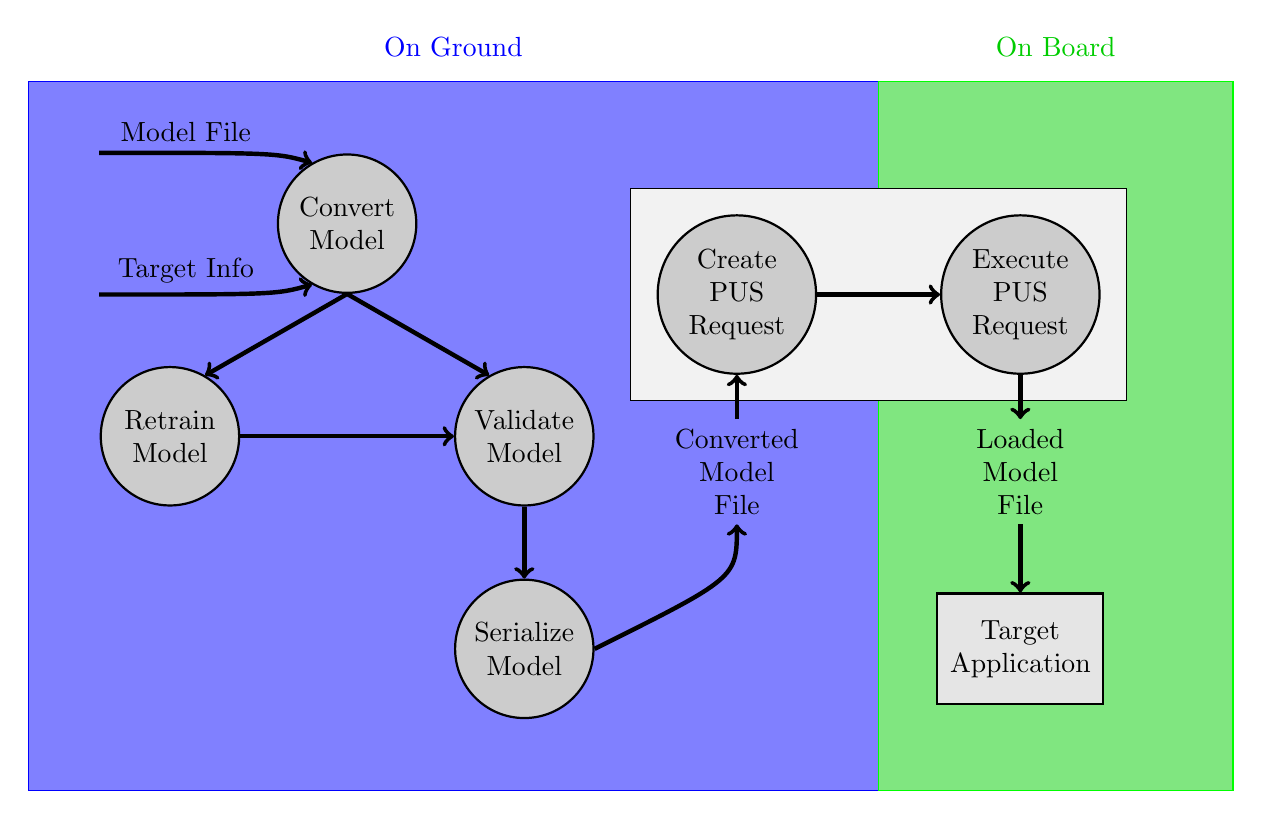
\begin{tikzpicture}[
	block/.style={
		circle,
		minimum size=5em,
		draw=black,
		thick,
		fill=black!20,
		align=center,
	},
	scale=0.9
]

\draw[color=blue, fill=blue!50] (-6,-5) rectangle (6,5);
\node[align=center,color=blue] at (0, 5.5) {On Ground};
\draw[color=green, fill=black!20!green!50] (6,-5) rectangle (11,5);
\node[align=center,color=black!20!green] at (8.5, 5.5) {On Board};

\draw[color=black, fill=black!5] (2.5,0.5) rectangle (9.5,3.5);

\node[block] (cm) at (-1.5,3) {Convert\\ Model};

\node[block] (rm) at (-4,0) {Retrain\\ Model};
\node[block] (vm) at (1,0) {Validate\\ Model};

\node[block] (sm) at (1,-3) {Serialize\\ Model};

\draw[->,ultra thick] (cm.south) -- (rm.60);
\draw[->,ultra thick] (cm.south) -- (vm.120);
\draw[->,ultra thick] (rm.east) -- (vm.west);
\draw[->,ultra thick] (vm.south) -- (sm.north);

\draw[->,ultra thick] (-5,4) .. node[pos=0.2, above] {Model File} controls (-2.5,4) .. (cm.120);
\draw[->,ultra thick] (-5,2) .. node[pos=0.2, above] {Target Info} controls (-2.5,2) .. (cm.240);

\node[block] (gpr) at (4,2) {Create\\ PUS\\ Request};
\node[align=center] (cmf) at (4,-0.5) {Converted\\ Model\\ File};
\draw[->,ultra thick] (sm.east) .. controls (4,-2) .. (cmf.south);
\draw[->,ultra thick] (cmf.north) -- (gpr.south);

\node[block] (epr) at (8,2) {Execute\\ PUS\\ Request};
\draw[->,ultra thick] (gpr.east) -- (epr.west);

\node[align=center] (lmf) at (8,-0.5) {Loaded\\ Model\\ File};
\node[align=center,thick,rectangle,draw=black,fill=black!10, minimum width=6em, minimum height=4em] (ta) at (8,-3) {Target\\ Application};

\draw[->,ultra thick] (epr.south) -- (lmf.north);
\draw[->,ultra thick] (lmf.south) -- (ta.north);

\end{tikzpicture}

\caption{Model Training, Transfer and Execution Framework.}
\label{f:model_framework}
\end{figure}

\section{Ground Training and Serialization}
Essentially, a framework should enable the creation of models in various ways with different libraries. This model file would need to be translated to a more general format, to be able to retrain with new data and to validate it. But with Tensorflow one can skip this step for now and lay the focus not on different architectures and libraries, but on handling the model itself. \newline
This means, a model needs to be trained with existing data, then validated and finally serialized. In the chapter before the training and validation of different Tensorflow models was already shown. The next step here is to serialize the model, to fit it into a machine readable byte array, which can be uploaded via telecommands onto a satellite.

The small, serialized format in Tensorflow is the so called \enquote{flatbuffer}. The flatbuffer only contains the most necessary information about the converted neural network. This includes only the structure and weights. \newline
To convert a neural network, it first has to be converted to a tf-lite model in an intermediate step. Unfortunately in Tensorflow Lite, not all kinds of neural networks are fully supported yet. The \acp{rnn} for example are still in an experimental state, hence the discussed \ac{lstm} will not be considered fully usable.

\section{Transfer and Upload}
The size of the converted neural network is rather small, in terms of storage. This can make updates rather easy. The \ac{pus} standard allows for a maximum package data size of $\SI{65535}{\byte}$. The tf-lite models created in the previous chapter did range from $\SI{10}{\kilo\byte}$ to $\SI{1}{\mega\byte}$. In the best case, the model is small enough to be uploaded within one package. In the worst case a model would need numerous consecutive packages. 

In the framework, this prerequisite helps to propose an additional \ac{pus} service for utilization of tf-lite models and machine learnings applications. This service has then the task to manage new models, model updates and the deletion of outdated models. A second task is to make these models available for other applications on board of the satellite.

\section{On-Board Execution}
For the model execution, a specific application has to be written. This application has to first verify the flatbuffer to prevent the execution of a corrupted model. The flatbuffer can verified once it is loaded into the memory. Then can be fed with new incoming data and executed to predict anomalies in the data.

The application on board of the \ac{spc} will be written in C/C++ as this corresponds to the language of the Tensorflow library and the flight software.